\documentclass{article}

\usepackage{hyperref}
\usepackage{booktabs}
\usepackage{tabularx}
\usepackage{graphicx}
\usepackage{float}

\title{SE 3XA3: SRS\\ohm Resistor Scanner}

\author{Team \# 4, ohm
		\\ Ryan Marks (marksr2)
		\\ Graeme Crawley (crawleg)
		\\ Jonathan Brown (brownjs2)
}


\date{}

%% Comments

\usepackage{color}

\newif\ifcomments\commentstrue

\ifcomments
\newcommand{\authornote}[3]{\textcolor{#1}{[#3 ---#2]}}
\newcommand{\todo}[1]{\textcolor{red}{[TODO: #1]}}
\else
\newcommand{\authornote}[3]{}
\newcommand{\todo}[1]{}
\fi

\newcommand{\wss}[1]{\authornote{blue}{SS}{#1}}
\newcommand{\ds}[1]{\authornote{red}{DS}{#1}}
\newcommand{\mj}[1]{\authornote{red}{MSN}{#1}}
\newcommand{\cm}[1]{\authornote{red}{CM}{#1}}
\newcommand{\mh}[1]{\authornote{red}{MH}{#1}}

% team members should be added for each team, like the following
% all comments left by the TAs or the instructor should be addressed
% by a corresponding comment from the Team

\newcommand{\tm}[1]{\authornote{magenta}{Team}{#1}}


\begin{document}

\begin{table}[hp]
\caption{Revision History} \label{TblRevisionHistory}
\begin{tabularx}{\textwidth}{llX}
\toprule
\textbf{Date} & \textbf{Developer(s)} & \textbf{Change}\\
\midrule
2016-09-26 & Ryan & Created template with section headings\\
... & ... & ...\\
\bottomrule
\end{tabularx}
\end{table}

\newpage

\maketitle



\section{Project Drivers}

\subsection{The Purpose of the Project }
The purpose of this project is to re-implement the open source package \href{https://github.com/sumeetkr/AndroidResistorScanner}{ "AndroidResistanceScanner" } by allowing a user to scan a standard resistor and output the resistance value to the screen, and then build upon that previously existing application by creating additional features and putting a greater emphasis on formal docuementation.

\subsection{The Stakeholders}
The main stakeholders for this application are the development team and our eventual users. However there are a number of different use cases for this application, so we will divide our users into the broad demographics of electronics beginners, colorblind hobbyists, and power users. Beginners are people new to electronics who dont know how to read resistor color codes and dont yet own a resistance meter to allow for measuring resistance rather than reading it. Another group that has difficulty reading resistor color codes are colorblind hobbyists. This particular set of people would benefit greatly as without this application they would have to rely on the word from those who are not color blind, or from the matching of shades. Finally power users who want to quickly find a resistor without manually searching, possibly with other use cases.

\section{Project Constraints}

\subsection{Mandated Constraints}
Constraints for this project can be broken into two categories; developer constraints and device constraints. Developer contraints are constraints that pertain to the development of the application while device constraints are constraints that pertain to the user's device and what is required to use the application. 
\subsubsection{Developer Constraints}
Developer constraints consist of the due date for the application which is December 7, 2016, the requirement that the application must be a re-implementation of a previously existing application on both Android and Windows, and the requirement that the application must be built at no cost to the developers.
\subsubsection{Device Constraints}
Device constraints include constraints on the hardware of the device and the resistors being scanned. Hardware constraints include the system having a camera and the CPU being fast enough to run the required algorithms. The resistors must be tan in colour and placed on a  flat, uniformly coloured surface.

\subsection{Naming Conventions and Terminology }
\begin{enumerate}
\item Resistor: Beige coloured, axial lead resistor
\item Device: The hardware running the application software
\item User: Any person who is using the final product to scan resistors
\item AndroidResistorScanner: The name of the open-source resistor scanning program
\end{enumerate}


\subsection{Relevant Facts and Assumptions}
It is assumed that the user knows the function of a resistor and understands how resistors are measured. It is also assumed that the user can see the text on the output screen. It is not assumed, however, that the user could read a resistor given a resistor chart.


\section{Functional Requirements}

\subsection{The Scope of the Work}

\subsubsection{The Current Situation}

Electronics hobbyists will use resistors in almost any project they encounter.
Currently there are a few ways they can identify the resistance of the resistors, these methods are as follows:
\begin{itemize}

\item Manual Method
\subitem The resistor colour code was developed to allow the ease of reading for people. 
With practise, people can quickly identify resistors by the colour bands, however this is less helpful when searching  for a specific resistor.
Additionally building proficiency takes time and can be a frustrating slowdown for a beginner, especially if they misidentify components during assembly.

\item Organizational Method
\subitem By storing resistors according to their resistances it becomes a trivial exercise to find a resistor of a given resistance.
This method is clearly superior in professional environments where very large numbers of resistors are on hand.

\item Meter Method
\subitem The current technique of choice for individuals who cannot discern colour codes is to measure a given resistor with a resistance meter.
This technique is immediately faster than reading colour bands, however it is somewhat laborious to have to pick up and test individual components.

\end{itemize}

\subsubsection{The Context of The Work}

This work has a very limited context, it serves as a tool to any person using colour band resistors who feels it useful.
There are not other subject matter domains that need to be understood or integrated with, beyond the resistor colour codes.

\subsubsection{Work Partitioning}

This work does not need to respond to any external business events, this section is not relevant

\subsection{Business Data Model \& Data Dictionary}

There is not a bussiness domain to be modelled by this software, as such these sections are not needed.

\subsection{The Scope of the Product}

\subsubsection{Product Boundary}
This project is a simple tool, with the user as the only actor.
As such the use case diagram is fairly minimal.

\begin{figure}[H]
    \includegraphics[width=0.8\textwidth]{UseCaseDiagram.png}
	\caption{The use case diagram for the system to be showing the product boundary.}
    \label{fig:use_case_diagram}
\end{figure}



\subsubsection{Product Use Cases}

As our products usability improves between phases of functionality, the use case will expand.
A use case for each phase is provided.

\textbf{ Phase 1 Use Case}

A user launches the app, and seeks to identify a specific resistor.
They hold the resistor up to the camera and aligns the primary axis resistor with an on screen line.
The system is constantly scanning, and once a coherent pattern of color bands is identified, the resistance is calculated and displayed.
Once the system can no longer identify a coherent pattern of color bands, the displayed resistance value dissappears, until a new resistor is identified.

\textbf{ Phase 2 Use Case}

A user launches the app, and seeks to identify a specific resistor.
The user points the camera in the general direction of the resistor, with little care for accurate framing.
The system is constantly scanning, and once a coherent pattern of color bands is identified, the resistance is calculated and displayed.
Once the system can no longer identify a coherent pattern of color bands, the displayed resistance value dissappears, until a new resistor is identified.

\textbf{ Phase 3 Use Case}

A user launches the app, and seeks to find a specific resistor in a group.
The user points the camera at the group of resistors.
The system is constantly scanning, and for any coherent pattern of color bands identified, the resistance is calculated and displayed in frame next to the resistor.

\subsection{Functional Requirements}

The functional requirements format given in the Volere template seems best suited to broad applications with many stakeholders and unclear development order.
For this document only the description, rationale, and fit criteria for a requirement will be given.
The requirements will be divided by the phases of development as meeting the goals of a given phase hinges on the completion of the ones before it.
There will not be a further prioritization of features beyond this phasing.

\subsubsection{ Phase 1 Functional Requirements}

\textbf{Description:} Display text over video stream
\\ \textbf{Rationale:} To meet the phase 1 use case, the resistance of the scanned resistor must be displayable.
\\ \textbf{Fit Criterion:} The criterion is exceedingly straightforward, if text can be displayed over the video stream, the requirement is met
\\ \\
\textbf{Description: } Identify the resistance of a resistor, two points indicating its primary axis.
\\ \textbf{Rationale: } In Phase 1 a line will be displayed over the video stream indicating where to position the resistor.
For greater modularity, and to allow for future phases to build on the source code, the scanning algorithm should work with an arbitrary defined or identified primary axis.
\\ \textbf{Fit Criterion:} This requirement shall be validated by testing it against human categorized resistors with a human annotated primary axis.
It shall have an accuracy as defined in the non-functional requirements.

\subsubsection{Phase 2 Functional Requirements}

\textbf{Description:} Identify the primary axis of a resistor arbitrarily positioned in an image. 
\\ \textbf{Rationale:} As is stated in the Phase 2 use case, we must be able to identify a resistor in any legible orientation.
The recognized primary axis shall be the same format and structure as is consumed by the resistance identification system so the two can be seamlessly integrated.
\\ \textbf{Fit Criterion: } This will be verified by running the algorithm against the human annotated primary axis.

\subsubsection{Phase 3 Functional Requirements}

\textbf{Description: } Identify the primary axis of many resistors arbitrarily positioned in an image. 
\\ \textbf{Rationale: } This is the necessary to meet the phase 3 use case that is not developed in an existing phase 
\\ \textbf{Fit Criterion: } This will be tested against a number of human annotated examples.
\\ \\
\textbf{Description: } Insert transformed text over a given primary axis.
\\ \textbf{Rationale: } By combining this subsystem with the scanning from phase 1 and axis identification in phase 3 we have the complete system to meet the phase 3 use case.
\\ \textbf{Fit Criterion: } This will be verified by having text sensibly displayed over the relevant axis of interest.


\section{Non-functional Requirements}

\subsection{Look and Feel Requirements }
\begin{enumerate}
\item The application shall have a very minimal user interface focussed primarily around the view of the camera.
\end{enumerate}
\subsection{Usability and Humanity Requirements}
\begin{enumerate}
\item The application shall be easily usable by people aged 8 to 70.
\item The application shall be suitable for a user with a minimal understanding of resistor colour codes and very little training.
\item The application shall not require the understanding of any particular language as all options symbolically.
\item The application shall be usable by those with colour blindness.
\end{enumerate}
\subsection{Performance Requirements}
\subsubsection{Speed and Latency Requirements}
\begin{enumerate}
\item The application should launch in no more than 5 seconds.
\item The algorithm used to process the income stream of images should be able to process between 15 and 30 images per second on a standard mobile phone.
\end{enumerate}
\subsubsection{Precision or Accuracy Requirements}
\begin{enumerate}
\item The application should identify an input as the correct class of resistor 95\% of the time.
\end{enumerate}
\subsubsection{Reliability and Availability Requirements}
\begin{enumerate}
\item The application will not require internet access.
\end{enumerate}
\subsection{Operational and Environmental Requirements}
\subsubsection{Expected Physical Environment}
\begin{enumerate}
\item The environment for the use of the application is in a household (hobyist) or light industrial setting.
\end{enumerate}
\subsubsection{Productization Requirements}
\begin{enumerate}
\item The application will be bundled as a .jar file for the desktop and as a .apk file for the Android platform.
\end{enumerate}
\subsubsection{Release Requirements}
\begin{enumerate}
\item The project will feature one pre-release demo with two full releases scheduled for November and December.
\end{enumerate}
\subsection{Maintainability and Support Requirements}
\begin{enumerate}
\item Once the product is launched, no further maintenance is required unless there is a desire for features to be added.
\item No live support for this product is necessary.
\item The application will support execution on the desktop and on Android.
\item The application might eventually be supported on iOS.
\end{enumerate}
\subsection{Security Requirements}
%\begin{enumerate}
The application does not possess any security concerns.
%\end{enumerate}
\subsection{Cultural Requirements}
The application does not feature any requirements specific to certain cultures outside of the usability requirements listed above.
\subsection{Legal Requirements}
\begin{enumerate}
\item The application should disclaim that it is not for use in safety critical systems.
\end{enumerate}

\section{Project Issues}

\subsection{Open Issues }
When it comes to scanning resistors, labelling them with their respective values is just the tip of the iceberg. The team would like to be able to scan a resistor of any size and colour against any surface, or scan by holding the resistor up to the camera. If possible, the application would also allow for a requested ohmage to be inputted and the combination of resistors needed would be highlighted.

\subsection{Off-the-Shelf Solutions}
There are many available applications to scan resistors and read resistor colour codes. A notable example is an application available on the Google Play store by the name of "Resistor Code Calculator" that allows a user to simply tap-to-highlight the coloured bands of the resistor in order and the app automatically calculates the resistance. The app doesn't solve the problem of colourblind users, but it solves the issue of reading a resistor in a much simpler way than our team's implementation. Similarly, many apps exist on app store that either allow the user to create a virtual circuit, or contain a large about of data about resistors that our application does not provide.

\subsection{New Problems}
There are currently none.

\subsection{Tasks}
See the Gantt chart below for an outline of tasks to be completed.
\begin{figure}[h]
\centering
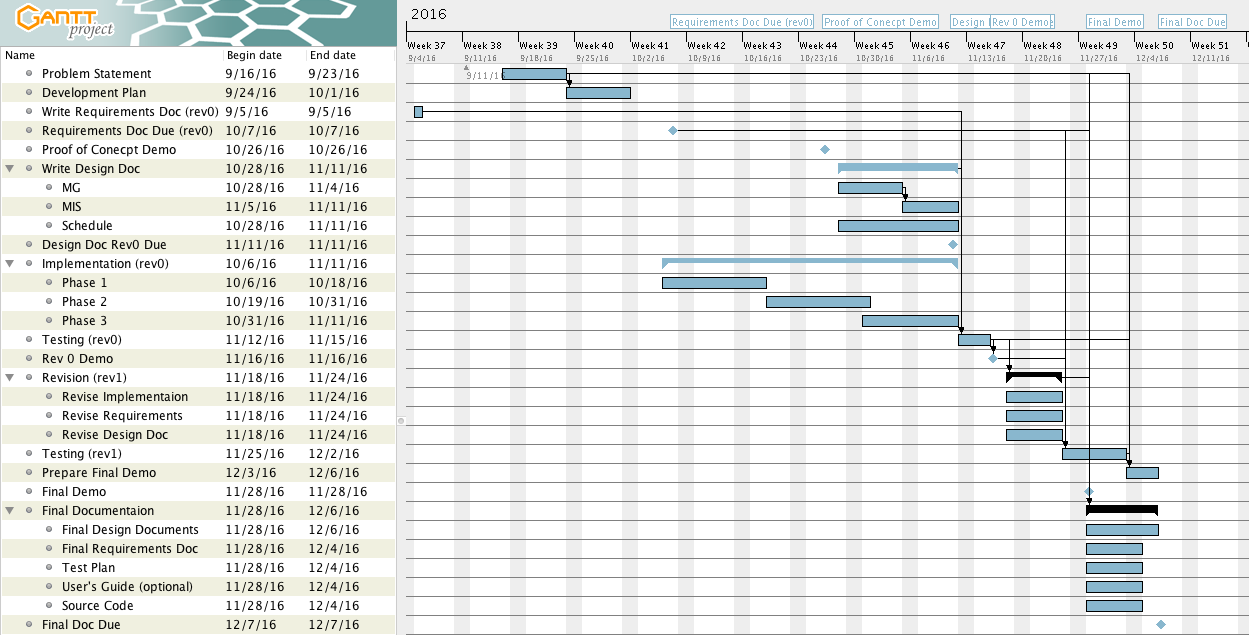
\includegraphics[scale=0.3]{gantt}
\end{figure}

\subsection{Migration to the New Product}
The product is designed in such a way that the core functionality of processing resistor data and outputing the value of the given resistor will never change. Instead, new features will be implemented in order of their priority, determined in the requirements section.

\subsection{Risks}
There are technical risks associated with building on the existing resistor product by including features such as the ability to scan multiple resistors at once, or find the requested resistor from an area containing multiple resistors. These risks are mitigated by having a phase-based development plan in which we start with the necessary base of the application and add new features that build on each other in each new phase.

\subsection{Costs}
The project contains no components that pose any cost to the development team.

\subsection{User Documentation and Training}
No training is required to use this application. A user guide will be available in the form of a popup menu when the app is first launched.

\subsection{Waiting Room}
See Phase 2 \& 3 Functional Requirements.

\subsection{Ideas for Solutions}
Using OpenCV, colours can be "binned" a small number of colours based on a range of RGB values. \\ 
ie: All colour swith low R, low G and medium to high B can be reduced to simply one shade of blue to make identification easier. \\



\end{document}